%!TEX root = mainfile.tex

\subsection{Including Recombinations} % (fold)
\label{sub:including_recombinations}

	To include Recombinations into our project, the rate at which hydrogen will recombine. The mean recombination time\cite{2012ApJ...746..125H} has the form
	\begin{align}
		\overline{t}_\text{rec}= \left[1.08\langle n_{H}\rangle\alpha_{B}C \right]^{-1}
	\end{align}
	Where $C$ is the clumping factor of the IGM (Section~\ref{sec:clumping_factor}), $\alpha_{B}$ is the recombination coefficent for excited states of hydrogen and the 1.08 accounts for the presence of photoelectrons from singly ionized helium.

	Values of the clumping factor against redshift are the ones used in Section~\ref{sec:clumping_factor}. The recombination coefficient for excited hydrogen is cited from\cite{1993PhyA..192..249L} and is proportional to $T_\text{IGM}^{-0.7}$ and at $T_\text{IGM}= 10^{4}$K it is equal to $2.6\times 10^{-13}$, therefore it is computed in the code as
	\begin{align}
		\alpha_{B}(T)(\si{\cubic\centi\metre\per\second}) &= \frac{2.6\times 10^{-13}*(10^{4})^{0.7}}{T^{0.7}}
	\end{align}
	However this also needs to be converted to \si{\cubic\mega\parsec} therefore we divide this equation by $(3.086\times 10^{24})^{3}$. Where the temperature of the IGM relation with redshift, derived from models\cite{2006MNRAS.373.1265O}, is
	\begin{align}
		T(z)=70047z^{-1.209}
	\end{align}
	To convert this into a rate of recombinations the code treats the recombinations as decays from hydrogen ionized state, with a lifetime of the mean recombination time. Then using the universal decay law the number of recombinations at a time, $t$, is
	\begin{align}
		n_{rec}(t)=n_\text{ion}(t)*\e{-t/\overline{t}_{rec}(t)}
	\end{align}
	Where we are taking $n_\text{ion}(t)$ to be the number of ionized hydrogen atoms at the time $t$. The code then does as it did in the previous cases but this time the fraction is
	\begin{align}
		X(z)=\frac{n_{ion}(z)-n_{rec}(z)}{n_{H}(z)}
	\end{align}
	This new outputted data is shown in Figure~\ref{fig:IonizedFraction3}.
	\begin{figure}[htbp]
		\centering
			\begingroup\endlinechar=-1
				\resizebox{0.7\textwidth}{!}{%
					% GNUPLOT: LaTeX picture with Postscript
\begingroup
  \makeatletter
  \providecommand\color[2][]{%
    \GenericError{(gnuplot) \space\space\space\@spaces}{%
      Package color not loaded in conjunction with
      terminal option `colourtext'%
    }{See the gnuplot documentation for explanation.%
    }{Either use 'blacktext' in gnuplot or load the package
      color.sty in LaTeX.}%
    \renewcommand\color[2][]{}%
  }%
  \providecommand\includegraphics[2][]{%
    \GenericError{(gnuplot) \space\space\space\@spaces}{%
      Package graphicx or graphics not loaded%
    }{See the gnuplot documentation for explanation.%
    }{The gnuplot epslatex terminal needs graphicx.sty or graphics.sty.}%
    \renewcommand\includegraphics[2][]{}%
  }%
  \providecommand\rotatebox[2]{#2}%
  \@ifundefined{ifGPcolor}{%
    \newif\ifGPcolor
    \GPcolortrue
  }{}%
  \@ifundefined{ifGPblacktext}{%
    \newif\ifGPblacktext
    \GPblacktexttrue
  }{}%
  % define a \g@addto@macro without @ in the name:
  \let\gplgaddtomacro\g@addto@macro
  % define empty templates for all commands taking text:
  \gdef\gplbacktext{}%
  \gdef\gplfronttext{}%
  \makeatother
  \ifGPblacktext
    % no textcolor at all
    \def\colorrgb#1{}%
    \def\colorgray#1{}%
  \else
    % gray or color?
    \ifGPcolor
      \def\colorrgb#1{\color[rgb]{#1}}%
      \def\colorgray#1{\color[gray]{#1}}%
      \expandafter\def\csname LTw\endcsname{\color{white}}%
      \expandafter\def\csname LTb\endcsname{\color{black}}%
      \expandafter\def\csname LTa\endcsname{\color{black}}%
      \expandafter\def\csname LT0\endcsname{\color[rgb]{1,0,0}}%
      \expandafter\def\csname LT1\endcsname{\color[rgb]{0,1,0}}%
      \expandafter\def\csname LT2\endcsname{\color[rgb]{0,0,1}}%
      \expandafter\def\csname LT3\endcsname{\color[rgb]{1,0,1}}%
      \expandafter\def\csname LT4\endcsname{\color[rgb]{0,1,1}}%
      \expandafter\def\csname LT5\endcsname{\color[rgb]{1,1,0}}%
      \expandafter\def\csname LT6\endcsname{\color[rgb]{0,0,0}}%
      \expandafter\def\csname LT7\endcsname{\color[rgb]{1,0.3,0}}%
      \expandafter\def\csname LT8\endcsname{\color[rgb]{0.5,0.5,0.5}}%
    \else
      % gray
      \def\colorrgb#1{\color{black}}%
      \def\colorgray#1{\color[gray]{#1}}%
      \expandafter\def\csname LTw\endcsname{\color{white}}%
      \expandafter\def\csname LTb\endcsname{\color{black}}%
      \expandafter\def\csname LTa\endcsname{\color{black}}%
      \expandafter\def\csname LT0\endcsname{\color{black}}%
      \expandafter\def\csname LT1\endcsname{\color{black}}%
      \expandafter\def\csname LT2\endcsname{\color{black}}%
      \expandafter\def\csname LT3\endcsname{\color{black}}%
      \expandafter\def\csname LT4\endcsname{\color{black}}%
      \expandafter\def\csname LT5\endcsname{\color{black}}%
      \expandafter\def\csname LT6\endcsname{\color{black}}%
      \expandafter\def\csname LT7\endcsname{\color{black}}%
      \expandafter\def\csname LT8\endcsname{\color{black}}%
    \fi
  \fi
  \setlength{\unitlength}{0.0500bp}%
  \begin{picture}(7200.00,4320.00)%
    \gplgaddtomacro\gplbacktext{%
      \put(747,595){\makebox(0,0)[r]{\strut{} 0}}%
      \put(747,1182){\makebox(0,0)[r]{\strut{} 0.2}}%
      \put(747,1768){\makebox(0,0)[r]{\strut{} 0.4}}%
      \put(747,2355){\makebox(0,0)[r]{\strut{} 0.6}}%
      \put(747,2942){\makebox(0,0)[r]{\strut{} 0.8}}%
      \put(747,3528){\makebox(0,0)[r]{\strut{} 1}}%
      \put(747,4115){\makebox(0,0)[r]{\strut{} 1.2}}%
      \put(849,409){\makebox(0,0){\strut{} 6}}%
      \put(1453,409){\makebox(0,0){\strut{} 8}}%
      \put(2058,409){\makebox(0,0){\strut{} 10}}%
      \put(2662,409){\makebox(0,0){\strut{} 12}}%
      \put(3267,409){\makebox(0,0){\strut{} 14}}%
      \put(3871,409){\makebox(0,0){\strut{} 16}}%
      \put(4475,409){\makebox(0,0){\strut{} 18}}%
      \put(5080,409){\makebox(0,0){\strut{} 20}}%
      \put(5684,409){\makebox(0,0){\strut{} 22}}%
      \put(6289,409){\makebox(0,0){\strut{} 24}}%
      \put(6893,409){\makebox(0,0){\strut{} 26}}%
      \csname LTb\endcsname%
      \put(144,2355){\rotatebox{-270}{\makebox(0,0){\strut{}Ionized Fraction}}}%
      \csname LTb\endcsname%
      \put(3871,130){\makebox(0,0){\strut{}Redshift ($z$)}}%
      \put(3871,4022){\makebox(0,0){\strut{}}}%
    }%
    \gplgaddtomacro\gplfronttext{%
      \csname LTb\endcsname%
      \put(5603,3729){\makebox(0,0)[r]{\strut{}Best Fit}}%
      \csname LTb\endcsname%
      \put(5603,3543){\makebox(0,0)[r]{\strut{}Lower Limit}}%
      \csname LTb\endcsname%
      \put(5603,3357){\makebox(0,0)[r]{\strut{}Upper Limit}}%
    }%
    \gplbacktext
    \put(0,0){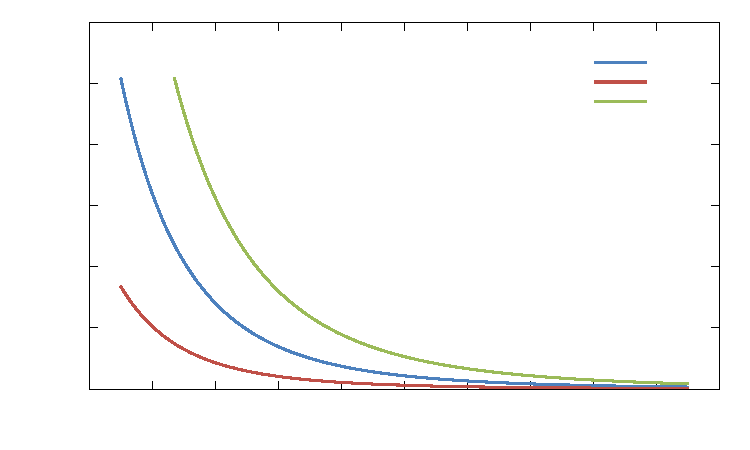
\includegraphics{GRAPH_recombinations}}%
    \gplfronttext
  \end{picture}%
\endgroup

				}\endgroup
		\caption{Ionized Fraction against redshift with recombinations and escape fraction included\label{fig:IonizedFraction3}}
	\end{figure}
	Which gives a redshift value of $7\pm1.8$ when fully ionized. This is still higher redshift than what we would expect it to be from the literature. This is probably mainly due to the large errors in value of the evolving escape fraction. Although it would appear that the first model is the most accurate in this regard it is not a very realistic number due to oversimplifying assumptions made.

	%talk about results
% subsection including_recombinations (end)



